\documentclass[12pt]{article}
\usepackage[margin = 1in]{geometry}
\usepackage[USenglish]{babel}
\usepackage{natbib}
\usepackage{multirow}
\usepackage{graphicx}
\usepackage{fancyhdr}
\usepackage{setspace}
\usepackage{verbatim}
\usepackage{booktabs}
\usepackage{amsmath}
\usepackage{lscape}
\usepackage{dcolumn}
\usepackage{subcaption}
\usepackage[title]{appendix}
\usepackage{xcolor}
\usepackage{todonotes}
\usepackage{titletoc}
\usepackage{longtable}
\usepackage[colorlinks=true,citecolor=red!50!black,urlcolor=blue!50!black,linkcolor=red!50!black]{hyperref}

% sans serif font
\renewcommand{\familydefault}{\sfdefault}

\title{{\large Online Appendix:}\\Measuring Morality in Political Attitude Expression}

%\author{Patrick W. Kraft\footnote{Ph.D. Candidate, Stony Brook University, \href{mailto:patrick.kraft@stonybrook.edu}{patrick.kraft@stonybrook.edu}.}}
\date{}

\begin{document}

%\footnotesize\singlespacing
\renewcommand\thesubsection{\Roman{subsection}}

\maketitle
\appendices
%\appendixpage
%Online appendices for manuscript: \\
%``Measuring Morality in Political Attitude Expression''

\thispagestyle{empty}
\startcontents[sections]
\printcontents[sections]{l}{1}{\setcounter{tocdepth}{2}}
\clearpage \setcounter{page}{1}

\begin{flushleft}\footnotesize
\section{Moral Foundations Dictionary}\label{app:dict}
\textit{Sources:}\\
\citet{graham2009liberals}, as well as \url{http://www.moralfoundations.org/}
\vspace{.5cm}

\textit{Note:}\\
Terms with (*) indicate that the word stem rather than the exact word was matched in the open-ended survey responses.
\vspace{.5cm}

\textbf{Care:}\\
safe*, peace*, compassion*, empath*, sympath*, care, caring, protect*, shield, shelter, amity, secur*, benefit*, defen*, guard*, preserve, harm*, suffer*, war, wars, warl*, warring, fight*, violen*, hurt*, kill, kills, killer*, killed, killing, endanger*, cruel*, brutal*, abuse*, damag*, ruin*, ravage, detriment*, crush*, attack*, annihilate*, destroy, stomp, abandon*, spurn, impair, exploit, exploits, exploited, exploiting, wound*
\vspace{.5cm}

\textbf{Fairness:}\\
fair, fairly, fairness, fair*, fairmind*, fairplay, equal*, justice, justness, justifi*, reciproc*, impartial*, egalitar*, rights, equity, evenness, equivalent, unbias*, tolerant, equable, balance*, homologous, unprejudice*, reasonable, constant, honest*, unfair*, unequal*, bias*, unjust*, injust*, bigot*, discriminat*, disproportion*, inequitable, prejud*, dishonest, unscrupulous, dissociate, preference, favoritism, segregat*, exclusion, exclud*
\vspace{.5cm}

\textbf{Loyalty:}\\
together, nation*, homeland*, family, families, familial, group, loyal*, patriot*, communal, commune*, communit*, communis*, comrad*, cadre, collectiv*, joint, unison, unite*, fellow*, guild, solidarity, devot*, member, cliqu*, cohort, ally, insider, foreign*, enem*, betray*, treason*, traitor*, treacher*, disloyal*, individual*, apostasy, apostate, deserted, deserter*, deserting, deceiv*, jilt*, imposter, miscreant, spy, sequester, renegade, terroris*, immigra*
\vspace{.5cm}

\textbf{Authority:}\\
obey*, obedien*, duty, law, lawful*, legal*, duti*, honor*, respect, respectful*, respected, respects, order*, father*, mother, motherl*, mothering, mothers, tradition*, hierarch*, authorit*, permit, permission, status*, rank*, leader*, class, bourgeoisie, caste*, position, complian*, command, supremacy, control, submi*, allegian*, serve, abide, defere*, defer, revere*, venerat*, comply, defian*, rebel*, dissent*, subver*, disrespect*, disobe*, sediti*, agitat*, insubordinat*, illegal*, lawless*, insurgent, mutinous, defy*, dissident, unfaithful, alienate, defector, heretic*, nonconformist, oppose, protest, refuse, denounce, remonstrate, riot*, obstruct
\vspace{.5cm}

\textbf{Sanctity:}\\
piety, pious, purity, pure*, clean*, steril*, sacred*, chast*, holy, holiness, saint*, wholesome*, celiba*, abstention, virgin, virgins, virginity, virginal, austerity, integrity, modesty, abstinen*, abstemiousness, upright, limpid, unadulterated, maiden, virtuous, refined, intemperate, decen*, immaculate, innocent, pristine, humble, disgust*, deprav*, disease*, unclean*, contagio*, indecen*, sin, sinful*, sinner*, sins, sinned, sinning, slut*, whore, dirt*, impiety, impious, profan*, gross, repuls*, sick*, promiscu*, lewd*, adulter*, debauche*, defile*, tramp, prostitut*, unchaste, wanton, profligate, filth*, trashy, obscen*, lax, taint*, stain*, tarnish*, debase*, desecrat*, wicked*, blemish, exploitat*, pervert, wretched*
\vspace{.5cm}

%\textbf{General:}\\
%righteous*, moral*, ethic*, value*, upstanding, good, goodness, principle*, blameless, exemplary, lesson, canon, doctrine, noble, worth*, ideal*, praiseworthy, commendable, character, proper, laudable, correct, wrong*, evil, immoral*, bad, offend*, offensive*, transgress*, honest*, lawful*, legal*, piety, pious, wholesome*, integrity, upright, decen*, indecen*, wicked*, wretched*

\end{flushleft}

\clearpage

\renewcommand\thefigure{\thesection.\arabic{figure}}
\renewcommand\thetable{\thesection.\arabic{table}}
\setcounter{figure}{0}
\setcounter{table}{0}

\section{Information on Data, Variables, and Recoding}

\subsection{Open-ended Responses and MFT Scores in 2012 ANES}

In this study, MFT scores are computed based on verbatim open-ended responses in which individuals describe what they \textit{liked} and \textit{disliked} about either presidential candidate as well as the Republican and Democratic parties. More specifically, respondents in the 2012 American National Election Study (ANES) were asked to list anything in particular that they like/dislike about the Democratic/Republican party as well as anything that might make them vote/not vote for either of the Presidential candidates and were probed by the interviewer asking ``anything else?'' until the respondent answered ``no''. All responses to the eight open-ended like/dislike questions (evaluating both parties and both candidates) were combined for each individual and pre-processed by correcting spelling errors using the Aspell spell checking algorithm (\url{www.aspell.net}).

% latex table generated in R 3.3.0 by xtable 1.8-2 package
% Fri Sep  2 15:41:09 2016
\begin{table}[ht]
\centering
\begin{tabular}{lcc}
  \hline
 & N & Percent \\ 
  \hline
Spanish Interview & 228 & 3.86 \\ 
  No Responses & 417 & 7.05 \\ 
   \hline
\end{tabular}
\caption{Missing open-ended responses} 
\label{tab:app_mis}
\end{table}


Respondents were not included in the analysis if they only provided extremely short responses (less or equal to 5 words in total), or if the interview language was Spanish. Table~\ref{tab:app_mis} provides an overview of the number of omitted cases. About 4\% of the interviews were held in Spanish and about 11\% of the respondents only provided extremely short or no responses (7\% did not answer any open-ended question). Furthermore, Figure~\ref{fig:appB2num} displays histograms of the length of the respondents' answers to all open-ended items. On average, the collection of all open-ended responses consists of about 75 words for each individual.

\begin{figure}[h]\centering
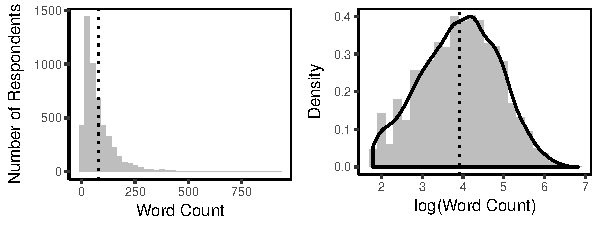
\includegraphics{../calc/fig/app_wc.pdf}
\caption{Histograms displaying the distribution of individual response lengths in number of words for each respective item category. Dotted lines indicate the average response length.}\label{fig:appB2num}
\end{figure}


Figure~\ref{fig:prop_ideol} presents the proportion of respondents who mentioned words that were included in the five different moral foundations dictionaries. Since responses for each individual represent their likes and dislikes across all eight open-ended items, each proportion indicates the percentage of individuals who mentioned a signal word belonging to the respective moral foundation in any of his or her open-ended responses evaluating the parties or candidates.

\begin{figure}[ht]\centering
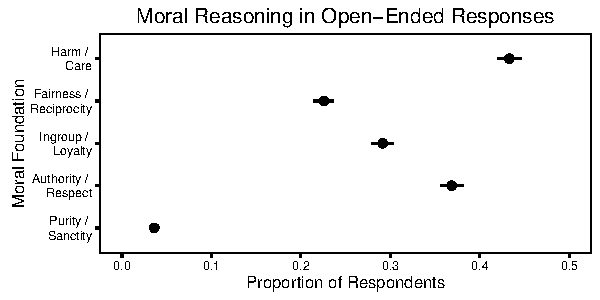
\includegraphics{../calc/fig/prop_mft.pdf}
\caption{Proportion of respondents mentioning each of the moral foundations in any of their open-ended responses, along with 95\% confidence intervals. The first two foundations are often labeled individualizing foundations, which have been shown to be more prevalent among liberals, while the remaining ones are described as binding foundations, which are more prevalent among conservatives.}\label{fig:prop_ideol}
\end{figure}
% ADD Note
% add note that first two are individualizing foundations, and the latter are binding foundations

The moral foundation most frequently mentioned is \textit{care}: About 40\% of the respondents mentioned at least one word included in respective dictionary. The second most frequently mentioned moral foundation is \textit{authority} with about 38\%. The proportion of respondents emphasizing \textit{loyalty} or \textit{fairness} is slightly lower with about 30\% and 23\%, respectively. \textit{Sanctity}, on the other hand, was almost never mentioned by any of the respondents, which suggests that the terms contained in the sanctity dictionary might be too uncommon in the context of politics and therefore not relevant for attitude expression. Due to the very rare mentioning of the sanctity dimension, the analyses in the main text concentrate on the remaining four moral foundations.\footnote{Unfortunately, this issue cannot not be addressed by relying on weighting scheme proposed in this study. The weights can correct for some distortions due to individual ubiquitous terms in the dictionaries, but it cannot compensate for the fact that the sanctity dictionary as a whole contains mostly words that are never mentioned by respondents.} Subsequent analyses focusing on the sanctity dimension in open-ended survey responses might necessitate a revision of the moral foundations dictionary. Overall, Figure~\ref{fig:prop_ideol} shows that a substantial proportion of individuals evokes moral considerations when describing their political attitudes even when they are not explicitly asked about morality.

The article proposes a weighting method to improve conventional dictionary approaches in order to capture the relative emphasis on each moral dimension (while correcting for ubiquitous terms and overall response length). Figure~\ref{fig:mft_weights} displays the weights used for each dictionary term that is mentioned at least once (terms that never appear are omitted). Terms that are very common, like ``care'', or ``foreign'', receive comparatively low weights. Such common terms are more likely to be used in multiple contexts and cannot be uniquely ascribed to the moral domain.\footnote{E.g., the statement ``I mostly care about foreign relations.'' should not be viewed as a moral argument.} On the other hand, dictionary terms that only appear in few responses are more likely to signal moral reasoning.

\begin{figure}[ht]\centering
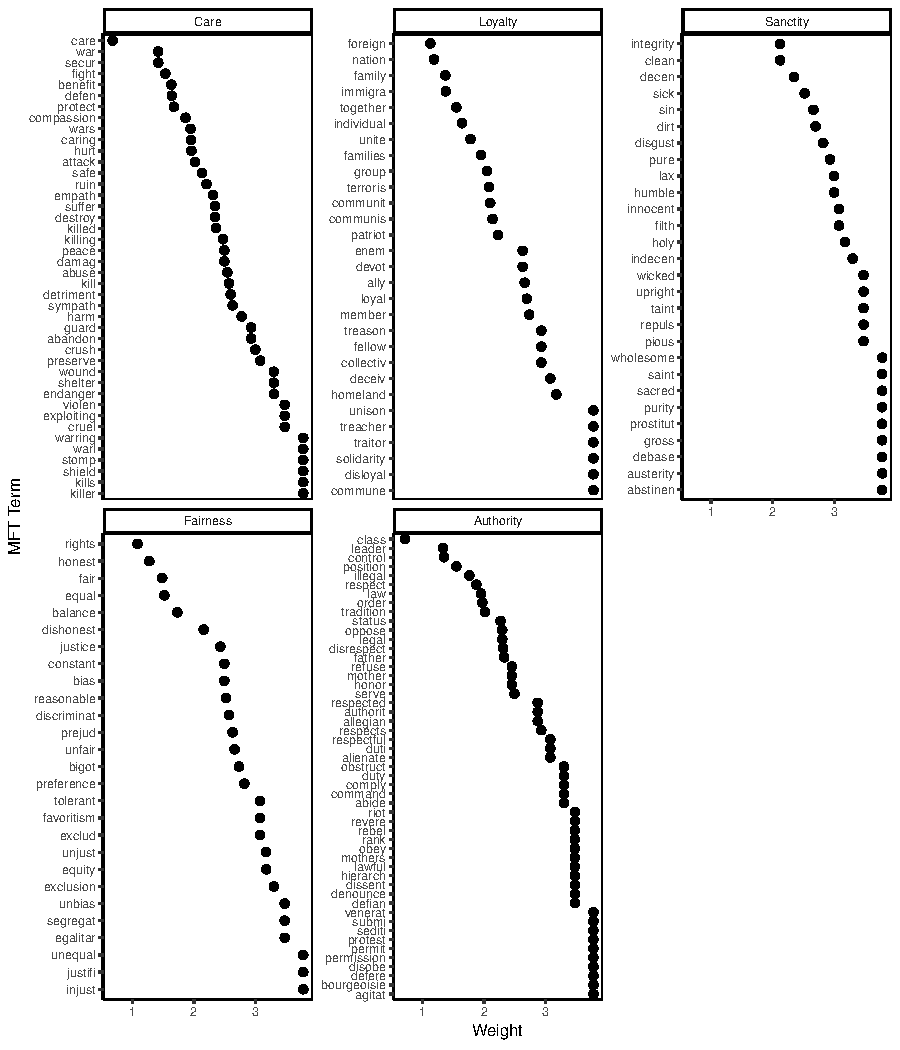
\includegraphics{../calc/fig/app_mftweights.pdf}
\caption{Weights for individual MFT dictionary terms (terms that were not mentioned by any respondent are excluded).}\label{fig:mft_weights}
\end{figure}

In parts of the analyses, MFT scores are combined to measure the overall reliance on moral considerations. This variable is computed as the sum of individual MFT scores across all dimensions (rescaled to unit variance after summation), which can be interpreted as a measure of general moralization in attitude expression.


\clearpage
\subsection{Moralization in Individual Media Environments}

The last analysis in the main text explores the effect of individual media environments on general moralization in political attitude expression. I make use of the fact that the 2012 ANES included a large array of items indicating whether individuals regularly watched various news outlets. For all media sources available, I downloaded the content of the coverage on either presidential candidates during the last month of the campaign (October 2012) from Lexis-Nexis and coded their emphasis on moral foundations using the same approach as for open-ended survey responses (general moralization). Figure~\ref{fig:media_desc} displays the resulting general MFT scores for each media outlet under consideration.

\begin{figure}[ht]\centering
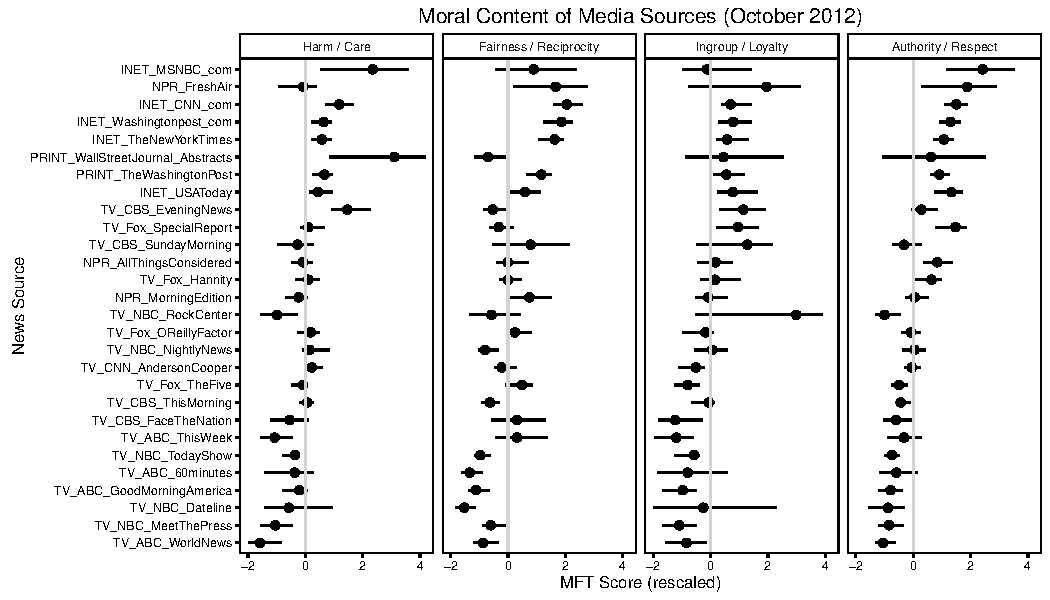
\includegraphics{../calc/fig/media_desc.pdf}
\caption{General MFT scores for media sources during 2012 U.S. Presidential campaign. Articles and scripts were selected if they mentioned either presidential candidate during the survey field period in the last month of the campaign (October). Contents were retrieved in full text from Lexis-Nexis (except for the Wall Street Journal, which only provided abstracts). Each media source was analyzed using the same procedure described for open-ended responses (median-centered and rescaled to unit variance). The figure also displays 95\% confidence intervals, which are based on parametric bootstraps of the document feature matrix of the entire corpus (1000 iterations).}\label{fig:media_desc}
\end{figure}


Based on the coded content for each media source, I created a measure that represents the extent to which each individual's media environment emphasized any moral foundation. For each respondent in the ANES, I select the media sources he or she reported to watch/read regularly and computed the mean of their respective MFT scores. Figure~\ref{fig:moralmedia} displays the histogram of the resulting variable. Individuals who did not report to have watched or read any of the media outlets were omitted from this analysis. Using this approach, I can analyze whether individuals who rely on media sources that emphasize moral foundations were also more likely to mention the moral considerations in their open-ended responses. 

\begin{figure}[ht]\centering
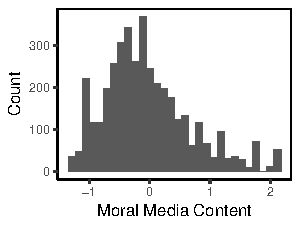
\includegraphics{../calc/fig/app_moralmedia.pdf}
\caption{Histogram of moralization in individual media environments. The variable is computed by averaging general MFT Scores for all media sources regularly consumed by each respondent.}\label{fig:moralmedia}
\end{figure}


\subsection{Remaining Variables in 2012 ANES}

The 2012 ANES contains two representative cross-sectional samples which are pooled in the analyses. One sample was collected via computer assisted face-to-face interviews while the other is based on an internet panel. Most items described below are drawn from the pre-election wave of the survey.\footnote{The open-ended items were included only in the pre-election wave. Accordingly, wherever possible, the set of explanatory variables was limited to the pre-election wave.} The key independent variable used to predict the emphasis on each moral foundation in the first step of the analyses is \textit{political ideology}. Respondents were asked to place themselves on a seven-point scale ranging from extremely liberal to extremely conservative, which was transformed into dichotomous indicators for respondents who identified as liberals, conservatives, or moderates. Additional control variables included in the analyses are \textit{age}, \textit{sex}, \textit{race} (African American), \textit{church attendance}, survey mode (online vs. offline), \textit{education} (college degree), as well as the overall length of the individual responses in the open-ended questions (\textit{measured as logged number of words}). Furthermore, the 2012 ANES included the \textit{Wordsum} vocabulary test as a measure of literacy and verbal skill. It consists of a series of items asking respondents to choose a term that is closest to a target word. The Wordsum score consists of an additive index of correct responses in ten individual trials. The inclusion of education, the length of individual responses, and the Wordsum score as control variables should account for potential confounding factors such as general effects of increased political literacy on the complexity of open-ended responses.

In order to examine the political relevance of moral reasoning measured through open-ended responses, the MFT scores for each moral foundation are used as independent variables to predict political outcomes. The dependent variable considered in the main text is \textit{voting behavior} (measured as a dichotomous indicator of vote choice for the Democratic rather than the Republican Presidential candidate reported in the post-election wave). Supplementary analyses in the appendix additionally examine \textit{candidate} and \textit{party evaluations}, each measured as the respective feeling thermometer differentials. In addition to the controls discussed previously, these analyses include measures of \textit{party identification}, which were recoded similarly to ideology.

The last step of the analyses investigates how the expression of moral considerations in political judgment is influenced by the content of individual media environments. Additional control variables in this step include \textit{political knowledge} (measured as the sum of correct answers to factual knowledge questions), \textit{political media exposure} (measured as the sum of weekly news consumption through TV, radio, internet, and print), and the frequency of \textit{political discussions} with friends and family members. As discussed in the main text, the analyses explore whether these factors influence \textit{general} moral reasoning. Figure~\ref{fig:app_desc} provides histograms of the variables included in each stage of the analyses. With the exception of age, all independent variables that were treated as continuous were rescaled to range from 0 to 1.

\begin{figure}[h]\centering
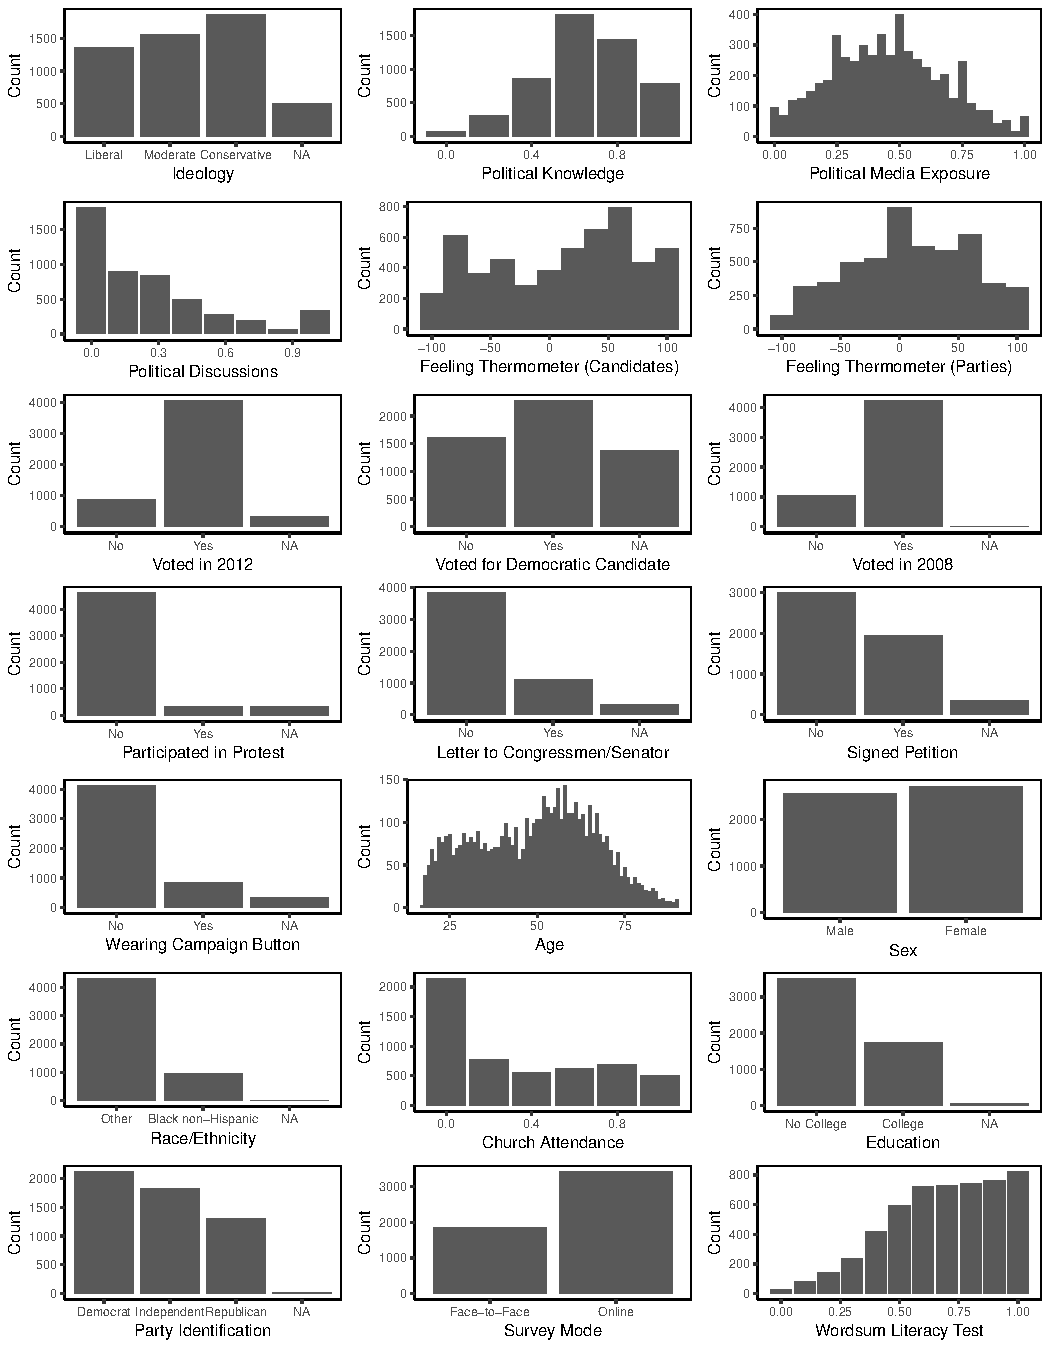
\includegraphics[width=\textwidth]{../calc/fig/app_desc.pdf}
\caption{Histograms for variables included in analyses.}\label{fig:app_desc}
\end{figure}


\clearpage
\subsection{Open-ended Responses and MFT Scores in Replication Sample}

The survey for the replication analysis was conducted via telephone with 594 adults aged 18 or older between early January, 2001 and July, 2003. The telephone numbers were a random-digit-dial (RDD) sample drawn from residents within a 25 mile radius of a large northeastern state university. As such, the survey was not conducted during a  major presidential election campaign and under a Republican presidency. Furthermore, the survey varied the set of open-ended items. Rather than asking about attitudes towards presidential candidates and both major parties, respondents were asked to describe liberals and conservatives as well as their respective beliefs in general:
\begin{itemize}
\item ``Can you briefly describe [liberals/conservatives] in your own words? What are they like?''
\item ``Can you briefly describe the political beliefs of [liberals/conservatives] in your own words? What do they believe?''
\end{itemize}
Based on these items, MFT scores were computed using the same procedures as for the 2012 ANES (i.e., pre-processing, weighting, etc.). Figure~\ref{fig:prop_lisurvey} displays the proportions of individuals in the replication dataset who mentioned each moral foundation in their open-ended response. Compared to the ANES sample (see Figure~\ref{fig:prop_ideol}), fewer individuals mentioned any of the foundations, which can be explained by the fact that the average response length in the telephone study is substantially shorter (28 words) than in the ANES (75 words). Notwithstanding, each of the foundations (except sanctity), was mentioned by between 10 and 20\% of the respondents.

\begin{figure}[ht]\centering
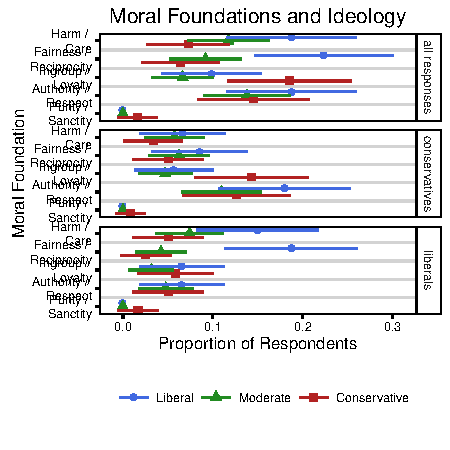
\includegraphics{../calc/fig/prop_lisurvey.pdf}
\caption{Proportion of respondents mentioning each of the moral foundations in any of their open-ended responses, along with 95\% confidence intervals in the replication dataset (RDD adult sample).}\label{fig:prop_lisurvey}
\end{figure}

\clearpage
\subsection{Control Variables in Replication Sample}

The coding of the remaining variables in the RDD survey is equivalent to those in the ANES analysis, although the survey did not contain the Wordsum scores (and varying survey mode) as additional controls. Histograms for all variables in the replication dataset are displayed in Figure~\ref{fig:app_lidesc}.


\begin{figure}[h]\centering
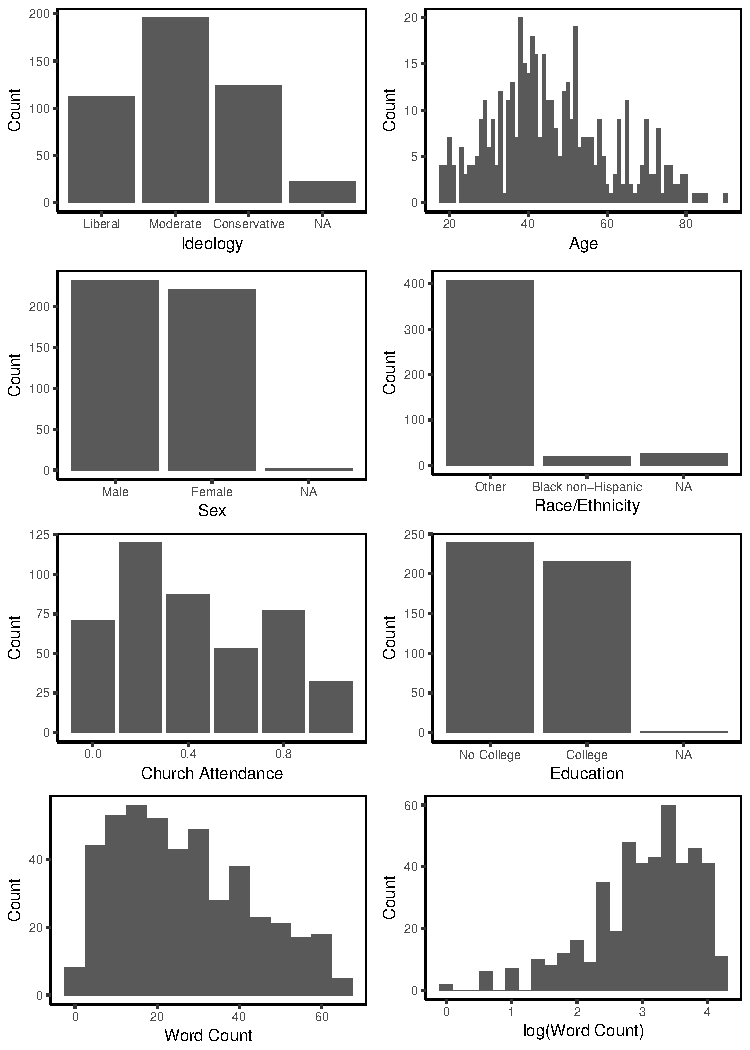
\includegraphics[width=.67\textwidth]{../calc/fig/app_lidesc.pdf}
\caption{Histograms for variables included in replication survey.}\label{fig:app_lidesc}
\end{figure}


\clearpage
\section{Additional Model Results \& Robustness Checks}\label{app:robust}
\renewcommand\thefigure{\thesection.\arabic{figure}}
\renewcommand\thetable{\thesection.\arabic{table}}
\setcounter{figure}{0}
\setcounter{table}{0}



\subsection{Replicating Ideological Differences using RDD Adult Sample}

The article raised the possibility that terms in the dictionary may coincidentally recover unrelated differences in word choice between liberals and conservatives when discussing their attitudes towards parties and candidates in the 2012 U.S. Presidential election. For example, one prominent issue in the election was the Affordable Care Act, which might increase the likelihood of Democrats mentioning the term ``care'' and thereby increasing the emphasis on the harm/care foundation irrespective of underlying moral considerations. In that case, observed ideological differences may be an artifact of the context in which the survey took place.

To address this concern, I replicated the analysis from Figure 1 in the article using data from a separate survey conducted via telephone with 594 adults aged 18 or older between early January, 2001 and July, 2003. The telephone numbers were a random-digit-dial (RDD) sample drawn from residents within a 25 mile radius of a large northeastern state university. The open-ended items asked respondents to describe liberals and conservatives as \textit{social groups} as well as their respective \textit{beliefs} in general. The coding and analyses are equivalent to those for Figure 1, although the survey did not contain the Wordsum scores included in the main analyses.

\begin{figure}[ht]\centering
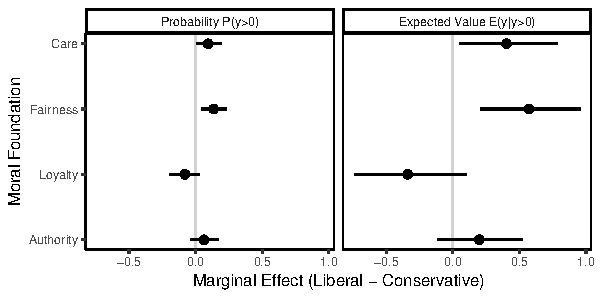
\includegraphics{../calc/fig/tobit_ideol_lisurvey.pdf}
\caption{Replication of main model (c.f., Figure 1) using RDD adult sample. Figure displays difference between liberals and conservatives in the probability of mentioning each moral foundation (left panel), and in the MFT score given that the foundation was mentioned (right panel), holding control variables at their respective means (along with 95\% confidence intervals). Control variables include church attendance, education, age, sex, race, and response length. Full model results are displayed in the appendix.
}\label{fig:tobit_ideol_lisurvey}
\end{figure}

Figure~\ref{fig:tobit_ideol_lisurvey} shows patterns that are consistent with previous results. Liberals are more likely to emphasize the foundations of care and fairness. The result for the loyalty dimension, however, do not reach conventional levels of statistical significance. Additional analyses reveal that the ideological differences in moral reasoning are mostly due to the fact that respondents who identify as liberals emphasize the foundations of care and fairness more strongly than conservatives when describing their ingroup (i.e., other liberals and their beliefs), while conservatives emphasize the loyalty foundation more strongly than liberals when describing their ingroup (results available upon request). The fact that the same basic ideological pattern can be recovered in a survey that was conducted in a different political context (non-election period, Republican administration), employed a different survey mode (phone interview), and relied on a different set of open-ended survey questions (asking about liberals and conservatives and their respective beliefs), provides additional evidence that the MFT dictionary recovers basic moral considerations in political attitude expression.



\subsection{Negations and Valence in Open-Ended Responses (2012 ANES)}

Dictionary-based approaches do not take into account the context in which signal terms appear. As such, they cannot capture directly whether individuals use certain words in a positive context or as part of a negation. Interpreting MFT scores as endorsements of a foundation might therefore be problematic if respondents commonly reject certain signal terms. Manual inspections of a random subset of open-ended suggested that most appearances of dictionary terms are not used in a direct negation (see also Table~\ref{tab:sample}). To provide a more comprehensive overview of potential negations or valenced statements in open-ended responses, I repeated the analyses from Figure 1 for different subsets of the questionnaire as well as the dictionary. The results are displayed in Figure~\ref{fig:tobit_ideol_app}.

\begin{figure}[ht]\centering
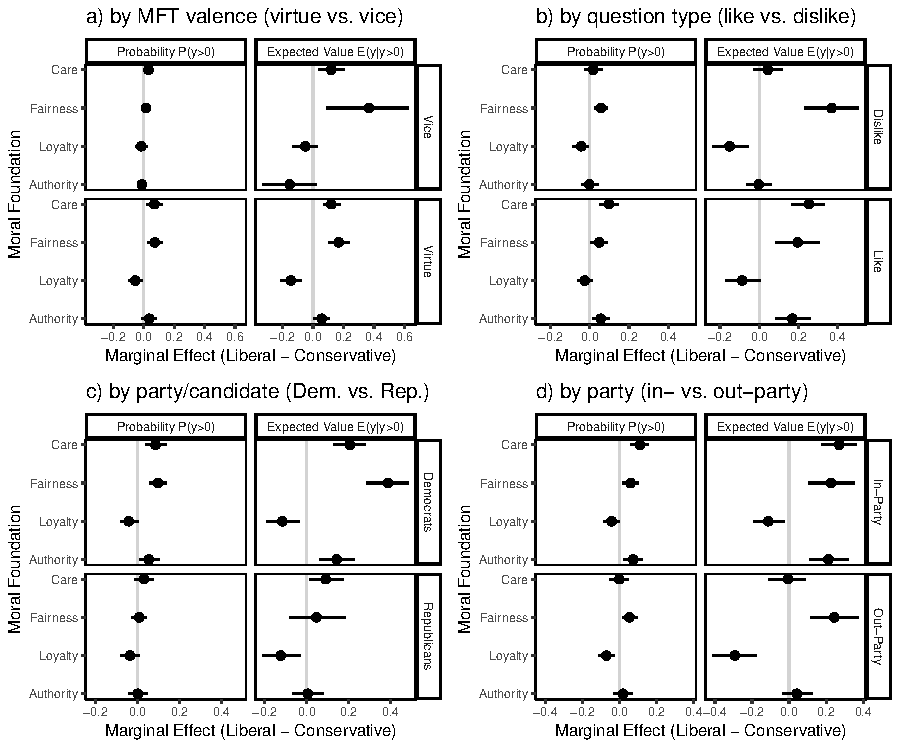
\includegraphics{../calc/fig/tobit_ideol_app.pdf}
\caption{Replication of main model (c.f., Figure~1) by different subgroups. The figure displays difference between liberals and conservatives in the probability of mentioning each moral foundation (left panel), and in the MFT score given that the foundation was mentioned (right panel), holding control variables at their respective means (along with 95\% confidence intervals). Control variables include church attendance, education, age, sex, race, and response length. Full model results are displayed in the appendix.
}\label{fig:tobit_ideol_app}
\end{figure}

Panel a) divides the MFT dictionary in positive and negative terms for each moral foundation (i.e. virtues and vices, c.f., \url{http://moralfoundations.org}) before examining ideological differences. Whether we only consider signal terms that represent ``vices'' (top) or ``virtues'' (bottom), the differences between liberals and conservatives in moral reasoning are largely consistent. Panel b) uses the full MFT dictionary again, but now splits up the set of open-ended questions before repeating the analysis. The top part displays the ideological differences when focusing on ``dislike'' questions, whereas the bottom part only considers ``like'' questions. While the results are again largely consistent, some interesting differences appear. For example, liberals are only more likely to emphasize the care foundation than conservatives when discussing issues they \textit{like} about parties and candidates, and not when they talk about things they \textit{dislike}. It seems unlikely that the consistent differences on ``Likes'' are driven by negations rather than positive endorsements of moral foundations. On the other hand, however, we also observe that liberals are more likely to emphasize the authority foundation than conservatives when talking about aspects they like. While this finding contradicts MFT, the remaining two panels provide some intuition about possible explanations. Panel c) splits up the open-ended responses by the party each respondent is asked to discuss. Here we observe that the ideological differences in moral reasoning are more pronounced when discussing the Democratic party and candidate as compared to the Republican party and candidate. A similar distinction is made in Panel d), where open-ended responses are divided into description of the respondent's respective out-party vs. in-party. Now, ideological differences appear to be more pronounced when respondents discuss their in-party rather than their out-party. Overall, regarding the surprising finding on authority, it appears that liberals where more likely to emphasize the foundation when discussing aspects that they like about their in-party candidate. A plausible example for such a pattern could be that they were more likely to describe the Democratic presidential candidate (Barack Obama) as a good ``leader'', which is a signal term for the authority dimension.


\clearpage
\subsection{MFT and Party/Candidate Evaluations (2012 ANES)}

The second part of the analyses in the main text examines whether the expression of moral foundations in open-ended responses is related to voting behavior. To further corroborate these results, I additionally examine the relationship of moral reasoning and attitudes towards political parties and candidates. Figure~\ref{fig:ols_feel} presents OLS estimates where feeling thermometer differentials between the Republican and the Democratic party (left panel) and between both Presidential candidates (right panel) are regressed on MFT scores for all moral foundations. 


\begin{figure}[ht]\centering
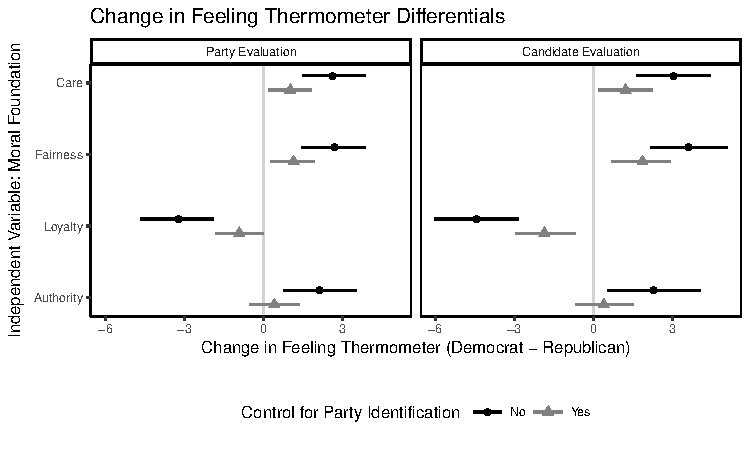
\includegraphics{../calc/fig/ols_feel.pdf}
\caption{Change in predicted feeling thermometer differential when MFT score is increased from its minimum (no overlap between dictionary and response) by one standard deviation, holding control variables constant at their respective means (along with 95\% confidence intervals). Positive values indicate that respondents who emphasized the respective foundation evaluated the Democratic candidate/party more favorably than the Republican candidate/party, and vice versa. Estimates are based on a single OLS model (using robust standard errors) including MFT scores for each foundation and gray triangles indicate estimates while additionally controlling for party identification. Remaining control variables are age, sex, race, church attendance, survey mode, education, response length, and the Wordsum vocabulary score.
% Full model results are displayed in Table~\ref{tab:ols_feel}.
}\label{fig:ols_feel}
\end{figure}

Positive values indicate more favorable evaluations for the Democratic candidate or party and negative values indicate more favorable evaluations of the Republican candidate or party. The patterns are consistent with previous results. Individuals who emphasize considerations related to care and fairness evaluate the Democratic party/candidate on average about 3 points higher than the Republican party/candidate (on a 100 point scale). On the other hand, if individuals emphasized the loyalty dimension, they reported stronger preferences for the Republican party/candidate. Interestingly, mentioning terms that belong to the authority dimension appears to increase favorability towards the democratic party and candidate, which contradicts MFT. However, the effect disappears once party identification is controlled for.

% ADD 2012 turnout?


\clearpage
\subsection{Other Correlates of General Moralization in Attitude Expression}

The last analysis in the article focuses on the effect of moralization in individual media environments on general moral reasoning in open-ended responses. Additional controls included in the model were political knowledge, general media exposure, and discussion frequency. Figure~\ref{fig:tobit_learn} allows for a comparison of effect sizes when each variable is increased from its empirical minimum value to its empirical maximum value, holding all other control variables constant at their means. To reiterate, the dependent variable captures the general tendency to emphasize \textit{any} moral foundation. Estimates are based on a Tobit model and the estimated effects are decomposed into the probability of mentioning any moral foundation (left panel) as well as the emphasis on morality, given that any foundation was mentioned (right panel).

\begin{figure}[h]\centering
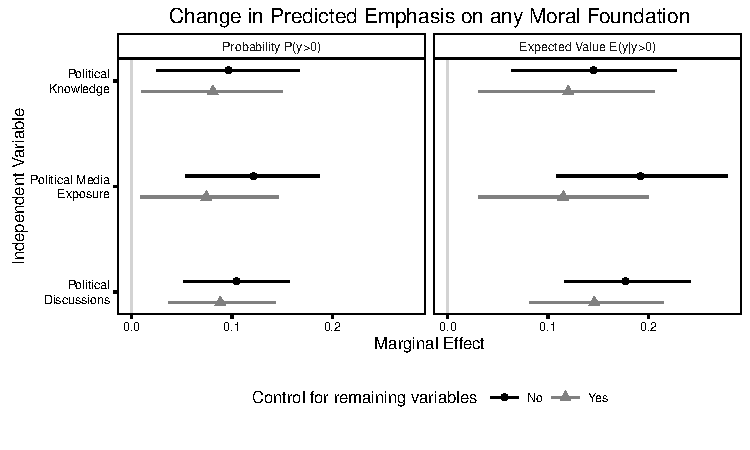
\includegraphics{../calc/fig/tobit_learn.pdf}
\caption{Change in predicted overall reliance on moral foundations depending on moral media content, political knowledge, media exposure, and frequency of political discussions. The plot shows differences in predicted probabilities of mentioning any moral foundation (left panel) as well as in the summed MFT scores given that any foundation was mentioned (right panel), if each of the independent variables is increased from its minimum to its maximum value holding all other variables constant at their respective means (along with 95\% confidence intervals). Additional control variables include age, sex, race, church attendance, survey mode, education, response length, and the Wordsum vocabulary score. 
%Full model results are displayed in the appendix, Table~\ref{tab:tobit_learn}.
}\label{fig:tobit_learn}
\end{figure}

The significant positive effect of frequent political discussions (even after controlling for moral media content, political knowledge, and media exposure), is especially interesting. Citizens who engage in frequent political arguments are more likely to use moral considerations when evaluating candidates and parties, which could suggest that morality serves as a rhetorical tool utilized to convince others of certain political views.


\subsection{Comparing General Media MFT Scores with Manual Coding}

The most fundamental concern related to the effects of individual media environments might be whether the content analysis of media sources using a dictionary is able to capture overall levels of moralization in news reporting. Luckily, a study reported in \citet{feinberg2013moral} included manual coding of a selection of newspaper articles on environmental issues to capture whether they use rhetoric grounded in each of the moral domains. Their coding therefore focuses on the same foundations without utilizing the dictionary. I computed a general moralization variable by summing the scores used in \citet{feinberg2013moral} and compared them to the MFT scores based on the procedures outlined above.\footnote{I am indebted to the authors for providing the data.}

\begin{figure}[ht]\centering
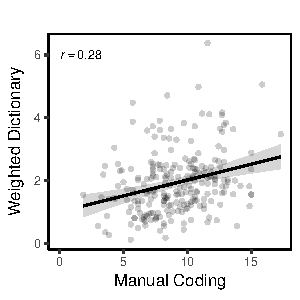
\includegraphics{../calc/fig/feinberg_general.pdf}
\caption{Validity check comparing general MFT Scores with individual coder assessments of newspaper articles in \citet{feinberg2013moral}.}\label{fig:ols_feinberg}
\end{figure}

Figure~\ref{fig:ols_feinberg} presents the correlation of general moralization in each article based on the manual coding in \citet{feinberg2013moral} compared to the dictionary method used in the analyses presented in the article. While the correlation is far from being perfect, the weighted dictionary method clearly captures some of the same variance as manual assessments of the emphasis on moral foundations. This is especially noteworthy since the coders in \citet{feinberg2013moral} did not rely on the moral foundations dictionary. This correspondence between subjective assessments and dictionary-based coding even persists when examining each moral foundation separately (c.f., Figure~\ref{fig:ols_feinberg_sep}).


\begin{figure}[ht]\centering
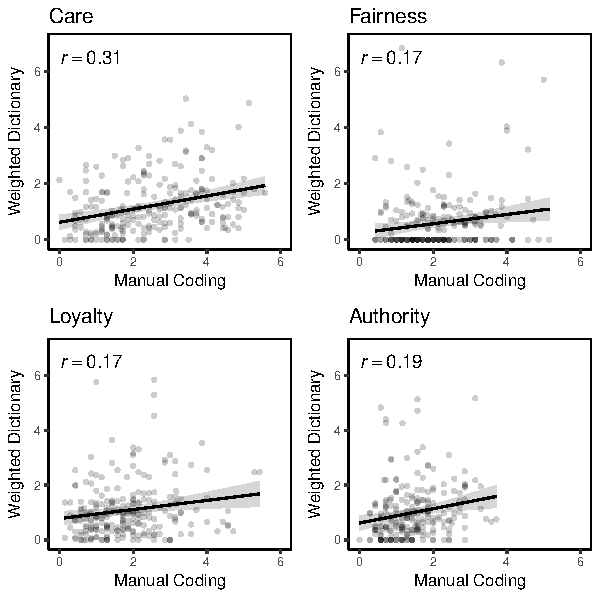
\includegraphics{../calc/fig/feinberg_sep.pdf}
\caption{Validity check comparing individual MFT Scores with individual coder assessments of newspaper articles in \citet{feinberg2013moral}.}\label{fig:ols_feinberg_sep}
\end{figure}



\clearpage
\subsection{Face Validity of Sample Response}

\begin{center} \small
\begin{longtable}{lp{2.7cm}p{5.5cm}p{5cm}}
\caption[Open-Ended Responses]{Sample of open-ended responses in the 2012 American National Election Study. Responses were selected if their length was within 10 words of average responses ($\sim75$ words) and if they scored high on one of the moral foundations (see first column). The second and third column display the item category and the raw response. The last column displays the processed response highlighting all signal words for the respective foundation.}\label{tab:sample} \\

\hline
	\textbf{Foundation} & \textbf{Variable} & \textbf{Raw Response} & \textbf{Processed Response} \\ \hline \endfirsthead
	
	\multicolumn{4}{c}{{\tablename\ \thetable{} -- continued from previous page}} \\
	\hline \textbf{Foundation} & \textbf{Variable} & \textbf{Raw Response} & \textbf{Processed Response} \\ \hline \endhead
	
	\hline \multicolumn{4}{r}{{Continued on next page}} \\	\endfoot
	
	\hline	\endlastfoot
	
	Care & Obama (like) & supports ending war, supports affordable health care for all, supports the preservation of medicare and social security, looking into energy conservation to preserve our planet for future generations, initiatives to promote education and job growth and much more. & \multirow{8}{5.5cm}{supports ending \textit{war} supports affordable health \textit{care} for all supports the preservation of medicare and social \textit{secur} looking into energy conservation to \textit{preserve} our planet for future generations initiatives to promote education and job growth and much more imposing a fine if someone does not get a health \textit{care} plan he supports a strong military anti same sex marriage anti women s choice for abortion not supportive of health \textit{care} reform act not sensitive to the needs of the very poor and immigra} \\
		 & Obama (dislike) & imposing a fine if someone does not get a health care plan \\
		 & Romney (like) & he supports a strong military \\
		 & Romney (dislike) & anti same sex marriage, anti women's choice for abortion, not supportive of health care reform act, not sensitive to the needs of the very poor and immigrants \\
		 & Dems (like) & -1 Inapplicable \\
		 & Dems (dislike) & -1 Inapplicable \\
		 & Reps (like) & -1 Inapplicable \\
		 & Reps (dislike) & -1 Inapplicable \\ \hline
	
	Fairness & Obama (like) & people rights, economy, taxes for working people, understanding of international problems & \multirow{8}{5.5cm}{people \textit{rights} economy taxes for working people understanding of international problems abortion \textit{rights} women \textit{rights} tax breaks for the rich military hawk rude and condescending to president obama economy women s \textit{rights} gay \textit{rights} health care tax plan for working class international strategy sometimes they do not fight hard enough against the republicans racist elitist trying to enrich the rich even more by hurt working people international relations health care women \textit{rights} gay \textit{rights}} \\
	 & Obama (dislike) & -1 Inapplicable \\
	 & Romney (like) & -1 Inapplicable \\
	 & Romney (dislike) & abortion rights, women rights, tax breaks for the rich, military hawk, rude and condescending to President Obama \\
	 & Dems (like) & economy, women's rights, gay rights, health care, tax plan for working class, international strategy. \\
	 & Dems (dislike) & sometimes they do not fight hard enough against the republicans. \\
	 & Reps (like) & -1 Inapplicable \\
	 & Reps (dislike) & racist, elitist, trying to enrich the rich even more by hurting working people, international relations, health care, women rights, gay rights \\ \hline	
	
	Loyalty & Obama (like) &  & \multirow{8}{5.5cm}{he dozen t do enough about keeping us safe from our \textit{foreign} \textit{enem} he s too iffy about isle too favorable about homosexuality abortion like his close \textit{family} ties good ideas about keeping us safe from \textit{foreign} countries strong on israel they support same sex marriage they won t bend i like the people that are their leader i vie nevier been disappointed in their positions on most things} \\
	 & Obama (dislike) & He doesn't do enough about keeping us safe from our foreign enemies; he's too iffy about Isael; too favorable about homosexuallity, abortion. \\
	 & Romney (like) & Like his close family ties; good ideas about keeping us safe from foreign countries; strong on Israel; \\
	 & Romney (dislike) &  \\
	 & Dems (like) &  \\
	 & Dems (dislike) & They support same sex marriage; they won't bend \\
	 & Reps (like) & I like the people that are their leaders; I've never been disappointed in their positions on most things. \\
	 & Reps (dislike) &  \\ \hline
	 
	 Authority & Obama (like) & competent, intelligent, but not strong in protecting US border, seriously dealing with illegal immigrant not rewarding for breaking the law. also, health care bill have me a little concern & \multirow{8}{5.5cm}{competent intelligent but not strong in protect us border seriously dealing with \textit{illegal} immigra not rewarding for breaking the \textit{law} also health care bill have me a little concern lack of strong laws dealing with \textit{illegal} aliens and us borders strong and firm dealing with foreign countries ie middle east china mexico the health care not too comfortable with what i am hearing about it} \\
	 	 & Obama (dislike) & lack of strong laws dealing with illegal aliens and US borders, strong and firm dealing with foreign countries ie middle east, china, mexico; the health care--not too comfortable with what I am hearing about it. \\
	 	 & Romney (like) & -1 Inapplicable \\
	 	 & Romney (dislike) & -1 Inapplicable \\
	 	 & Dems (like) & -1 Inapplicable \\
	 	 & Dems (dislike) & -1 Inapplicable \\
	 	 & Reps (like) & -1 Inapplicable \\
	 	 & Reps (dislike) & -1 Inapplicable \\
\end{longtable}
\end{center}



\clearpage
\section{Tables of Model Estimates}\label{app:tables}
\renewcommand\thefigure{\thesection.\arabic{figure}}
\renewcommand\thetable{\thesection.\arabic{table}}
\setcounter{figure}{0}
\setcounter{table}{0}


CONTENT FOLLOWS

%\subsection{Ideological Differences in Moral Reasoning}
%% latex table generated in R 3.3.3 by xtable 1.8-2 package
% Tue Mar 14 22:58:48 2017
\begin{table}[ht]
\centering
\caption{Tobit models predicting MFT score for each foundation based 
           on ideology. Positive coefficients indicate stronger emphasis on the respective 
           foundation. Standard errors in parentheses. Estimates are used for Figure 
           \ref{fig:tobit_ideol} in the main text.} 
\label{tab:tobit_ideol}
\begingroup\footnotesize
\begin{tabular}{lcccc}
  \hline
Variable & Harm & Fairness & Ingroup & Authority \\ 
  \hline
Ideology (Conservative) & -0.307 & -0.697 &  0.366 & -0.132 \\ 
   & (0.08) & (0.143) & (0.115) & (0.091) \\ 
  Ideology (Moderate) & -0.135 & -0.513 &  0.099 & -0.060 \\ 
   & (0.081) & (0.146) & (0.121) & (0.093) \\ 
  Church Attendance & -0.063 &  0.110 &  0.247 & -0.123 \\ 
   & (0.092) & (0.167) & (0.132) & (0.105) \\ 
  Education (College Degree) & -0.093 &  0.237 &  0.308 &  0.106 \\ 
   & (0.07) & (0.125) & (0.099) & (0.079) \\ 
  Age &  0.002 &  0.001 & -0.007 &  0.003 \\ 
   & (0.002) & (0.004) & (0.003) & (0.002) \\ 
  Sex (Female) &  0.133 &  0.078 & -0.245 & -0.095 \\ 
   & (0.063) & (0.114) & (0.091) & (0.072) \\ 
  Race (African American) &  0.045 & -0.125 & -0.215 &  0.338 \\ 
   & (0.091) & (0.166) & (0.135) & (0.101) \\ 
  Word Count (log) &  0.364 &  0.527 &  0.773 &  0.584 \\ 
   & (0.033) & (0.061) & (0.051) & (0.039) \\ 
  Wordsum Score &  0.562 &  0.661 &  0.604 &  0.324 \\ 
   & (0.166) & (0.302) & (0.241) & (0.188) \\ 
  Survey Mode (Online) & -0.039 &  0.205 &  0.149 &  0.300 \\ 
   & (0.076) & (0.138) & (0.109) & (0.087) \\ 
  Intercept & -2.506 & -4.742 & -4.857 & -3.617 \\ 
   & (0.193) & (0.363) & (0.297) & (0.226) \\ 
  log(Sigma) &  0.553 &  1.025 &  0.868 &  0.684 \\ 
   & (0.021) & (0.027) & (0.023) & (0.02) \\ 
   \hline
N & 4684 & 4684 & 4684 & 4684 \\ 
  Log-Likelihood & -4924 & -3961 & -4567 & -5043 \\ 
   \hline
\end{tabular}
\endgroup
\end{table}

%
%\clearpage
%\subsection{The Political Relevance of Moral Reasoning}
%% latex table generated in R 3.3.3 by xtable 1.8-2 package
% Tue Mar 14 22:58:48 2017
\begin{table}[h]
\centering
\caption{OLS models predicting feeling thermometer differentials based on
           MFT score for each foundation. Positive coefficients indicate more favorable evaluation 
           of Democratic candidate/party than the Republican candidate/party, and vice versa. 
           Standard errors in parentheses. Estimates are used for Figure \ref{fig:ols_feel} 
           in the main text.} 
\label{tab:ols_feel}
\begingroup\footnotesize
\begin{tabular}{lcccc}
  \hline
Variable & Party (1) & Party (2) & Cand. (1) & Cand. (2) \\ 
  \hline
Harm &   2.558 &   0.781 &   2.798 &   0.907 \\ 
   & (0.714) & (0.5) & (0.855) & (0.642) \\ 
  Fairness &   1.833 &   0.692 &   3.095 &   1.793 \\ 
   & (0.623) & (0.435) & (0.748) & (0.56) \\ 
  Ingroup &  -2.919 &  -0.900 &  -4.009 &  -1.767 \\ 
   & (0.647) & (0.452) & (0.777) & (0.583) \\ 
  Authority &   2.214 &   0.503 &   2.209 &   0.338 \\ 
   & (0.669) & (0.468) & (0.796) & (0.597) \\ 
  PID (Democrat) &  &  44.602 &  &  47.207 \\ 
   &  & (1.074) &  & (1.375) \\ 
  PID (Republican) &  & -44.706 &  & -52.275 \\ 
   &  & (1.189) &  & (1.527) \\ 
  Church Attendance & -27.658 & -11.449 & -35.883 & -17.639 \\ 
   & (1.82) & (1.296) & (2.18) & (1.666) \\ 
  Education (College Degree) &   0.310 &   1.311 &   1.361 &   2.525 \\ 
   & (1.464) & (1.023) & (1.756) & (1.317) \\ 
  Age &  -0.109 &  -0.119 &  -0.307 &  -0.316 \\ 
   & (0.039) & (0.028) & (0.047) & (0.035) \\ 
  Sex (Female) &   7.475 &   2.939 &   9.280 &   4.383 \\ 
   & (1.279) & (0.897) & (1.532) & (1.152) \\ 
  Race (African American) &  52.935 &  20.983 &  63.106 &  28.211 \\ 
   & (1.739) & (1.294) & (2.08) & (1.659) \\ 
  Word Count (log) &   2.308 &   1.089 &   1.758 &   0.335 \\ 
   & (0.636) & (0.445) & (0.762) & (0.571) \\ 
  Wordsum Score &  -0.862 &   2.579 &   0.553 &   4.125 \\ 
   & (3.297) & (2.309) & (3.955) & (2.971) \\ 
  Survey Mode (Online) &  -5.829 &  -1.986 &  -8.684 &  -4.467 \\ 
   & (1.511) & (1.06) & (1.808) & (1.362) \\ 
  Intercept &   8.242 &   4.708 &  21.501 &  19.260 \\ 
   & (3.346) & (2.385) & (4.002) & (3.056) \\ 
   \hline
N & 5135 & 5123 & 5151 & 5140 \\ 
  R-squared (adj.) & 0.211 & 0.616 & 0.224 & 0.565 \\ 
   \hline
\end{tabular}
\endgroup
\end{table}

%% latex table generated in R 3.4.2 by xtable 1.8-2 package
% Sat Nov 25 14:03:51 2017
\begin{table}[ht]
\centering
\caption{Logit models predicting democratic vote choice based on
           MFT score for each foundation. Positive coefficients indicate higher likelihood
           to vote for the Democratic candidate than the Republican candidate. Standard errors 
           in parentheses. Estimates are used for Figure 2 in the main text.} 
\label{tab:logit_vote}
\begingroup\footnotesize
\begin{tabular}{lcc}
  \hline
Variable & (1) & (2) \\ 
  \hline
Harm &  0.192 &  0.171 \\ 
   & (0.043) & (0.061) \\ 
  Fairness &  0.170 &  0.129 \\ 
   & (0.041) & (0.053) \\ 
  Ingroup & -0.190 & -0.068 \\ 
   & (0.041) & (0.054) \\ 
  Authority &  0.076 &  0.025 \\ 
   & (0.041) & (0.056) \\ 
  PID (Democrat) &  &  2.618 \\ 
   &  & (0.136) \\ 
  PID (Republican) &  & -2.676 \\ 
   &  & (0.156) \\ 
  Church Attendance & -1.614 & -1.352 \\ 
   & (0.113) & (0.158) \\ 
  Education (College Degree) &  0.155 &  0.370 \\ 
   & (0.085) & (0.119) \\ 
  Age & -0.009 & -0.017 \\ 
   & (0.002) & (0.003) \\ 
  Sex (Female) &  0.275 &  0.160 \\ 
   & (0.078) & (0.108) \\ 
  Race (African American) &  4.229 &  3.234 \\ 
   & (0.263) & (0.288) \\ 
  Word Count (log) &  0.145 &  0.116 \\ 
   & (0.044) & (0.061) \\ 
  Wordsum Score &  0.048 &  0.174 \\ 
   & (0.21) & (0.29) \\ 
  Survey Mode (Online) & -0.366 & -0.388 \\ 
   & (0.095) & (0.131) \\ 
  Intercept &  0.313 &  0.509 \\ 
   & (0.238) & (0.328) \\ 
   \hline
N & 3706 & 3698 \\ 
  Log-Likelihood & -1955 & -1138 \\ 
   \hline
\end{tabular}
\endgroup
\end{table}

%
%\clearpage
%\subsection{The Conditionality of Moral Reasoning}
%% latex table generated in R 3.3.0 by xtable 1.8-2 package
% Thu Nov 10 12:04:38 2016
\begin{table}[ht]
\centering
\caption{Tobit models predicting overall reliance on moral foundations
           (sum of MFT scores) based on political knowledge, media exposure, and frequency of 
           political discussions. Positive coefficients indicate stronger emphasis on any foundation.
           Standard errors in parentheses. Estimates are used for Figure \ref{fig:tobit_learn} in 
           the main text.} 
\label{tab:tobit_learn}
\begingroup\footnotesize
\begin{tabular}{lcccc}
  \hline
Variable & (1) & (2) & (3) & (4) \\ 
  \hline
Political Knowledge &  0.260 &  &  &  0.236 \\ 
   & (0.098) &  &  & (0.103) \\ 
  Political Media Exposure &  &  0.369 &  &  0.272 \\ 
   &  & (0.088) &  & (0.095) \\ 
  Political
Discussions &  &  &  0.263 &  0.202 \\ 
   &  &  & (0.068) & (0.07) \\ 
  Church Attendance & -0.020 & -0.022 & -0.006 & -0.010 \\ 
   & (0.052) & (0.053) & (0.055) & (0.055) \\ 
  Education (College Degree) &  0.079 &  0.079 &  0.097 &  0.070 \\ 
   & (0.043) & (0.042) & (0.044) & (0.044) \\ 
  Age & -0.001 & -0.002 &  0.000 & -0.002 \\ 
   & (0.001) & (0.001) & (0.001) & (0.001) \\ 
  Sex (Female) &  0.018 &  0.016 &  0.017 &  0.041 \\ 
   & (0.037) & (0.037) & (0.038) & (0.039) \\ 
  Race (African American) &  0.109 &  0.088 &  0.082 &  0.091 \\ 
   & (0.05) & (0.05) & (0.052) & (0.052) \\ 
  Word Count (log) &  0.099 &  0.097 &  0.090 &  0.080 \\ 
   & (0.019) & (0.018) & (0.019) & (0.02) \\ 
  Wordsum Score &  0.281 &  0.353 &  0.323 &  0.257 \\ 
   & (0.1) & (0.096) & (0.1) & (0.104) \\ 
  Survey Mode (Online) &  0.042 &  0.043 &  0.099 &  0.061 \\ 
   & (0.044) & (0.044) & (0.046) & (0.047) \\ 
  Intercept & -0.401 & -0.380 & -0.356 & -0.446 \\ 
   & (0.1) & (0.097) & (0.101) & (0.105) \\ 
  log(Sigma) &  0.209 &  0.209 &  0.213 &  0.212 \\ 
   & (0.014) & (0.014) & (0.014) & (0.014) \\ 
   \hline
N & 5173 & 5164 & 4834 & 4827 \\ 
  Log-Likelihood & -7132 & -7117 & -6687 & -6672 \\ 
   \hline
\end{tabular}
\endgroup
\end{table}

%% latex table generated in R 3.3.3 by xtable 1.8-2 package
% Sun Mar 19 13:46:11 2017
\begin{table}[ht]
\centering
\caption{Tobit models predicting MFT score for each foundation based 
           on political knowledge (mean-centered) and ideology. Positive coefficients indicate stronger 
           emphasis on the respective foundation. Standard errors in parentheses. Estimates are used 
           for Figure \ref{fig:tobit_ideol_know} in the main text.} 
\label{tab:tobit_ideol_know}
\begingroup\footnotesize
\begin{tabular}{lcccc}
  \hline
Variable & Harm & Fairness & Ingroup & Authority \\ 
  \hline
Political Knowledge &  0.795 & -0.236 & -0.037 &  0.882 \\ 
   & (0.299) & (0.472) & (0.406) & (0.312) \\ 
  Ideology (Conservative) & -0.325 & -0.866 &  0.340 & -0.092 \\ 
   & (0.092) & (0.152) & (0.123) & (0.096) \\ 
  Knowledge * Conservative & -0.984 &  0.780 &  0.551 & -0.596 \\ 
   & (0.388) & (0.632) & (0.511) & (0.4) \\ 
  Ideology (Moderate) & -0.190 & -0.730 &  0.044 & -0.003 \\ 
   & (0.091) & (0.15) & (0.125) & (0.095) \\ 
  Knowledge * Moderate & -0.503 &  0.653 &  0.136 & -1.077 \\ 
   & (0.405) & (0.667) & (0.552) & (0.417) \\ 
  Church Attendance &  0.014 &  0.066 &  0.255 & -0.105 \\ 
   & (0.103) & (0.169) & (0.134) & (0.105) \\ 
  Education (College Degree) & -0.129 &  0.280 &  0.328 &  0.078 \\ 
   & (0.079) & (0.128) & (0.102) & (0.08) \\ 
  Age &  0.000 &  0.001 & -0.008 &  0.002 \\ 
   & (0.002) & (0.004) & (0.003) & (0.002) \\ 
  Sex (Female) &  0.107 &  0.139 & -0.204 & -0.088 \\ 
   & (0.071) & (0.118) & (0.094) & (0.073) \\ 
  Race (African American) &  0.123 & -0.033 & -0.236 &  0.353 \\ 
   & (0.101) & (0.169) & (0.139) & (0.102) \\ 
  Word Count (log) &  0.410 &  0.601 &  0.751 &  0.492 \\ 
   & (0.041) & (0.068) & (0.055) & (0.042) \\ 
  Wordsum Score &  0.659 &  0.721 &  0.547 &  0.221 \\ 
   & (0.193) & (0.321) & (0.256) & (0.197) \\ 
  Survey Mode (Online) & -0.054 &  0.294 &  0.130 &  0.266 \\ 
   & (0.085) & (0.141) & (0.112) & (0.088) \\ 
  Intercept & -2.575 & -4.962 & -4.664 & -3.133 \\ 
   & (0.236) & (0.403) & (0.325) & (0.246) \\ 
  log(Sigma) &  0.669 &  1.045 &  0.884 &  0.683 \\ 
   & (0.02) & (0.026) & (0.022) & (0.02) \\ 
   \hline
N & 4489 & 4489 & 4489 & 4489 \\ 
  Log-Likelihood & -5144 & -3983 & -4579 & -5025 \\ 
   \hline
\end{tabular}
\endgroup
\end{table}

%% latex table generated in R 3.3.2 by xtable 1.8-2 package
% Mon Feb 27 15:07:15 2017
\begin{table}[ht]
\centering
\caption{Tobit models predicting MFT score for each foundation based 
           on political media exposure (mean-centered) and ideology. Positive coefficients indicate 
           stronger emphasis on the respective foundation. Standard errors in parentheses. Estimates 
           are used for Figure \ref{fig:tobit_ideol_media} in the main text.} 
\label{tab:tobit_ideol_media}
\begingroup\footnotesize
\begin{tabular}{lcccc}
  \hline
Variable & Harm & Fairness & Ingroup & Authority \\ 
  \hline
Political Media Exposure &  0.557 &  0.113 &  0.678 &  0.773 \\ 
   & (0.262) & (0.46) & (0.394) & (0.302) \\ 
  Ideology (Conservative) & -0.281 & -0.731 &  0.379 & -0.123 \\ 
   & (0.081) & (0.146) & (0.117) & (0.093) \\ 
  Media * Conservative & -0.651 &  0.811 & -0.385 & -0.177 \\ 
   & (0.341) & (0.606) & (0.491) & (0.388) \\ 
  Ideology (Moderate) & -0.122 & -0.508 &  0.121 & -0.034 \\ 
   & (0.081) & (0.146) & (0.122) & (0.093) \\ 
  Media * Moderate & -0.383 &  0.041 & -0.507 & -0.691 \\ 
   & (0.35) & (0.629) & (0.525) & (0.402) \\ 
  Church Attendance & -0.066 &  0.113 &  0.249 & -0.124 \\ 
   & (0.092) & (0.167) & (0.132) & (0.105) \\ 
  Education (College Degree) & -0.108 &  0.226 &  0.293 &  0.079 \\ 
   & (0.07) & (0.126) & (0.1) & (0.079) \\ 
  Age &  0.001 & -0.001 & -0.009 &  0.000 \\ 
   & (0.002) & (0.004) & (0.003) & (0.002) \\ 
  Sex (Female) &  0.139 &  0.102 & -0.231 & -0.069 \\ 
   & (0.063) & (0.115) & (0.092) & (0.072) \\ 
  Race (African American) &  0.032 & -0.122 & -0.217 &  0.322 \\ 
   & (0.091) & (0.167) & (0.135) & (0.102) \\ 
  Word Count (log) &  0.359 &  0.520 &  0.765 &  0.576 \\ 
   & (0.033) & (0.061) & (0.051) & (0.039) \\ 
  Wordsum Score &  0.563 &  0.650 &  0.623 &  0.322 \\ 
   & (0.166) & (0.302) & (0.242) & (0.188) \\ 
  Survey Mode (Online) & -0.049 &  0.189 &  0.132 &  0.284 \\ 
   & (0.076) & (0.139) & (0.11) & (0.088) \\ 
  Intercept & -2.445 & -4.616 & -4.762 & -3.480 \\ 
   & (0.199) & (0.371) & (0.305) & (0.232) \\ 
  log(Sigma) &  0.553 &  1.025 &  0.868 &  0.684 \\ 
   & (0.021) & (0.027) & (0.023) & (0.02) \\ 
   \hline
N & 4678 & 4678 & 4678 & 4678 \\ 
  Log-Likelihood & -4916 & -3955 & -4561 & -5034 \\ 
   \hline
\end{tabular}
\endgroup
\end{table}

%% latex table generated in R 3.3.0 by xtable 1.8-2 package
% Thu Nov 10 12:04:39 2016
\begin{table}[ht]
\centering
\caption{Tobit models predicting MFT score for each foundation based 
           on political discussion frequency (mean-centered) and ideology. Positive coefficients 
           indicate stronger emphasis on the respective foundation. Standard errors in parentheses. 
           Estimates are used for Figure \ref{fig:tobit_ideol_disc} in the main text.} 
\label{tab:tobit_ideol_disc}
\begingroup\footnotesize
\begin{tabular}{lcccc}
  \hline
Variable & Harm & Fairness & Ingroup & Authority \\ 
  \hline
Political Discussion &  0.149 &  0.182 &  0.178 &  0.222 \\ 
   & (0.182) & (0.341) & (0.282) & (0.216) \\ 
  Ideology (Conservative) & -0.283 & -0.727 &  0.276 & -0.122 \\ 
   & (0.079) & (0.153) & (0.12) & (0.094) \\ 
  Discussion * Conservative &  0.132 &  0.683 &  0.717 &  0.242 \\ 
   & (0.238) & (0.45) & (0.356) & (0.28) \\ 
  Ideology (Moderate) & -0.157 & -0.497 &  0.090 & -0.090 \\ 
   & (0.079) & (0.153) & (0.124) & (0.094) \\ 
  Discussion * Moderate & -0.356 &  0.729 &  0.576 & -0.547 \\ 
   & (0.27) & (0.507) & (0.41) & (0.322) \\ 
  Church Attendance &  0.001 &  0.126 &  0.265 & -0.149 \\ 
   & (0.09) & (0.174) & (0.135) & (0.106) \\ 
  Education (College Degree) & -0.074 &  0.222 &  0.308 &  0.119 \\ 
   & (0.068) & (0.13) & (0.101) & (0.08) \\ 
  Age & -0.002 &  0.000 & -0.007 &  0.003 \\ 
   & (0.002) & (0.004) & (0.003) & (0.002) \\ 
  Sex (Female) &  0.158 &  0.124 & -0.240 & -0.070 \\ 
   & (0.061) & (0.119) & (0.093) & (0.073) \\ 
  Race (African American) &  0.003 & -0.135 & -0.228 &  0.338 \\ 
   & (0.088) & (0.173) & (0.138) & (0.103) \\ 
  Word Count (log) &  0.311 &  0.474 &  0.730 &  0.557 \\ 
   & (0.033) & (0.064) & (0.053) & (0.04) \\ 
  Wordsum Score &  0.530 &  0.698 &  0.550 &  0.342 \\ 
   & (0.162) & (0.317) & (0.249) & (0.192) \\ 
  Survey Mode (Online) & -0.079 &  0.251 &  0.219 &  0.283 \\ 
   & (0.074) & (0.145) & (0.113) & (0.089) \\ 
  Intercept & -1.972 & -4.605 & -4.670 & -3.526 \\ 
   & (0.188) & (0.383) & (0.308) & (0.234) \\ 
  log(Sigma) &  0.509 &  1.033 &  0.856 &  0.665 \\ 
   & (0.021) & (0.028) & (0.023) & (0.021) \\ 
   \hline
N & 4377 & 4377 & 4377 & 4377 \\ 
  Log-Likelihood & -4812 & -3727 & -4271 & -4726 \\ 
   \hline
\end{tabular}
\endgroup
\end{table}

%% latex table generated in R 3.3.0 by xtable 1.8-2 package
% Thu Nov 10 12:04:39 2016
\begin{table}[ht]
\centering
\caption{Tobit models predicting MFT score for each foundation based 
           on moral content of individual media environments. Positive coefficients 
           indicate stronger emphasis on the respective foundation. Standard errors in parentheses. 
           Estimates are used for Figure \ref{fig:tobit_cont} in the main text.} 
\label{tab:tobit_cont}
\begingroup\footnotesize
\begin{tabular}{lcccc}
  \hline
Variable & Harm & Fairness & Ingroup & Authority \\ 
  \hline
Media MFT score (harm) &  0.030 &  &  &  \\ 
   & (0.016) &  &  &  \\ 
  Media MFT score (fairness) &  &  0.051 &  &  \\ 
   &  & (0.024) &  &  \\ 
  Media MFT score (ingroup) &  &  &  0.001 &  \\ 
   &  &  & (0.029) &  \\ 
  Media MFT score (authority) &  &  &  &  0.001 \\ 
   &  &  &  & (0.017) \\ 
  Church Attendance & -0.128 & -0.029 &  0.357 & -0.115 \\ 
   & (0.078) & (0.152) & (0.124) & (0.097) \\ 
  Education (College Degree) & -0.063 &  0.239 &  0.345 &  0.110 \\ 
   & (0.063) & (0.122) & (0.099) & (0.079) \\ 
  Age & -0.002 &  0.002 & -0.004 &  0.001 \\ 
   & (0.002) & (0.003) & (0.003) & (0.002) \\ 
  Sex (Female) &  0.196 &  0.153 & -0.308 & -0.092 \\ 
   & (0.055) & (0.109) & (0.088) & (0.069) \\ 
  Race (African American) &  0.161 & -0.020 & -0.272 &  0.383 \\ 
   & (0.073) & (0.15) & (0.123) & (0.092) \\ 
  Word Count (log) &  0.304 &  0.560 &  0.798 &  0.588 \\ 
   & (0.028) & (0.058) & (0.049) & (0.037) \\ 
  Wordsum Score &  0.519 &  0.679 &  0.452 &  0.255 \\ 
   & (0.143) & (0.288) & (0.233) & (0.181) \\ 
  Survey Mode (Online) & -0.117 &  0.322 &  0.248 &  0.268 \\ 
   & (0.064) & (0.128) & (0.104) & (0.081) \\ 
  Intercept & -2.025 & -5.414 & -4.945 & -3.535 \\ 
   & (0.152) & (0.331) & (0.269) & (0.201) \\ 
  log(Sigma) &  0.481 &  1.011 &  0.879 &  0.691 \\ 
   & (0.019) & (0.026) & (0.022) & (0.019) \\ 
   \hline
N & 5173 & 5173 & 5173 & 5173 \\ 
  Log-Likelihood & -5650 & -4222 & -4936 & -5581 \\ 
   \hline
\end{tabular}
\endgroup
\end{table}

%
%\clearpage
%\subsection{Examining Alternative Explanations}
%% latex table generated in R 3.3.0 by xtable 1.8-2 package
% Thu Nov  3 19:42:25 2016
\begin{table}[ht]
\centering
\caption{Tobit models predicting MFT score for each foundation based 
           on ideology (telephone survey replication). Positive coefficients indicate stronger emphasis on the respective 
           foundation. Standard errors in parentheses. Estimates are used for Figure 
           \ref{fig:tobit_ideol_lisurvey} in the main text.} 
\label{tab:tobit_ideol_lisurvey}
\begingroup\footnotesize
\begin{tabular}{lcccc}
  \hline
Variable & Harm & Fairness & Ingroup & Authority \\ 
  \hline
Ideology (Conservative) &  -2.451 & -3.497 &   1.786 & -0.993 \\ 
   & (1.102) & (1.196) & (1.123) & (0.808) \\ 
  Ideology (Moderate) &  -1.374 & -1.917 &  -1.394 & -1.030 \\ 
   & (0.876) & (0.859) & (1.096) & (0.687) \\ 
  Church Attendance &  -0.918 &  1.363 &   1.015 &  1.455 \\ 
   & (1.282) & (1.25) & (1.375) & (0.977) \\ 
  Education (College Degree) &   0.810 &  0.482 &   1.197 &  1.100 \\ 
   & (0.787) & (0.762) & (0.885) & (0.606) \\ 
  Age &  -0.002 &  0.044 &  -0.031 & -0.058 \\ 
   & (0.026) & (0.025) & (0.029) & (0.022) \\ 
  Sex (Female) &  -0.777 & -0.097 &  -0.706 & -0.400 \\ 
   & (0.774) & (0.753) & (0.853) & (0.587) \\ 
  Race (African American) &   0.591 &  1.563 &  -0.038 &  0.385 \\ 
   & (1.731) & (1.598) & (2.107) & (1.305) \\ 
  Word Count (log) &   2.517 &  0.269 &   1.562 &  0.728 \\ 
   & (0.671) & (0.481) & (0.645) & (0.399) \\ 
  Intercept & -11.759 & -7.623 & -10.262 & -3.802 \\ 
   & (2.794) & (2.249) & (2.803) & (1.652) \\ 
  log(Sigma) &   1.507 &  1.433 &   1.595 &  1.325 \\ 
   & (0.121) & (0.139) & (0.127) & (0.108) \\ 
   \hline
N & 395 & 395 & 395 & 395 \\ 
  Log-Likelihood & -224 & -192 & -219 & -266 \\ 
   \hline
\end{tabular}
\endgroup
\end{table}

%
%\clearpage
%\subsection{Additional Models and Robustness Checks in Appendix}
%% latex table generated in R 3.3.0 by xtable 1.8-2 package
% Thu Nov  3 16:40:24 2016
\begin{table}[ht]
\centering
\caption{Tobit models predicting overall reliance on moral foundations
           (sum of MFT scores) based on political participation. Positive coefficients indicate 
           stronger emphasis on any foundation. Standard errors in parentheses. Estimates are 
           used for Figure \ref{fig:tobit_part} in the appendix.} 
\label{tab:tobit_part}
\begingroup\footnotesize
\begin{tabular}{lcccccc}
  \hline
Variable & (1) & (2) & (3) & (4) & (5) & (6) \\ 
  \hline
Voted in 2008 &  0.096 &  &  &  &  &  0.091 \\ 
   & (0.052) &  &  &  &  & (0.054) \\ 
  Protest &  &  0.076 &  &  &  & -0.002 \\ 
   &  & (0.076) &  &  &  & (0.08) \\ 
  Petition &  &  &  0.122 &  &  &  0.091 \\ 
   &  &  & (0.041) &  &  & (0.044) \\ 
  Button &  &  &  &  0.135 &  &  0.106 \\ 
   &  &  &  & (0.051) &  & (0.052) \\ 
  Letter &  &  &  &  &  0.090 &  0.040 \\ 
   &  &  &  &  & (0.048) & (0.051) \\ 
  Church Attendance & -0.032 &  0.001 &  0.001 & -0.007 & -0.004 & -0.023 \\ 
   & (0.053) & (0.055) & (0.055) & (0.055) & (0.055) & (0.055) \\ 
  Education (College Degree) &  0.085 &  0.103 &  0.095 &  0.108 &  0.095 &  0.086 \\ 
   & (0.043) & (0.044) & (0.044) & (0.044) & (0.044) & (0.045) \\ 
  Age & -0.001 &  0.000 &  0.000 &  0.000 &  0.000 & -0.001 \\ 
   & (0.001) & (0.001) & (0.001) & (0.001) & (0.001) & (0.001) \\ 
  Sex (Female) &  0.002 &  0.011 &  0.010 &  0.010 &  0.015 &  0.014 \\ 
   & (0.037) & (0.038) & (0.038) & (0.038) & (0.038) & (0.039) \\ 
  Race (African American) &  0.089 &  0.088 &  0.090 &  0.069 &  0.092 &  0.071 \\ 
   & (0.05) & (0.052) & (0.052) & (0.052) & (0.052) & (0.053) \\ 
  Word Count (log) &  0.103 &  0.105 &  0.097 &  0.103 &  0.101 &  0.091 \\ 
   & (0.018) & (0.019) & (0.019) & (0.019) & (0.019) & (0.02) \\ 
  Wordsum Score &  0.339 &  0.349 &  0.312 &  0.350 &  0.338 &  0.299 \\ 
   & (0.096) & (0.1) & (0.101) & (0.1) & (0.1) & (0.101) \\ 
  Survey Mode (Online) &  0.053 &  0.080 &  0.070 &  0.073 &  0.069 &  0.056 \\ 
   & (0.044) & (0.045) & (0.046) & (0.045) & (0.046) & (0.046) \\ 
  Intercept & -0.353 & -0.385 & -0.362 & -0.376 & -0.358 & -0.364 \\ 
   & (0.097) & (0.101) & (0.102) & (0.101) & (0.102) & (0.103) \\ 
  log(Sigma) &  0.209 &  0.215 &  0.215 &  0.214 &  0.214 &  0.213 \\ 
   & (0.014) & (0.014) & (0.014) & (0.014) & (0.014) & (0.014) \\ 
   \hline
N & 5157 & 4846 & 4833 & 4849 & 4847 & 4816 \\ 
  Log-Likelihood & -7108 & -6709 & -6688 & -6709 & -6709 & -6657 \\ 
   \hline
\end{tabular}
\endgroup
\end{table}

%% latex table generated in R 3.3.3 by xtable 1.8-2 package
% Tue Mar 14 22:58:50 2017
\begin{table}[ht]
\centering
\caption{Tobit models predicting MFT score for each foundation based 
           on political knowledge, media exposure, and discussion frequency (all mean-centered)
           as well as ideology. Positive coefficients indicate stronger emphasis on the respective
           foundation. Standard errors in parentheses. Estimates are used for Figure
           \ref{fig:tobit_ideol_difdif} in the appendix.} 
\label{tab:tobit_ideol_difdif}
\begingroup\footnotesize
\begin{tabular}{lcccc}
  \hline
Variable & Harm & Fairness & Ingroup & Authority \\ 
  \hline
Political Knowledge &  0.671 & -0.188 & -0.093 &  0.789 \\ 
   & (0.28) & (0.492) & (0.407) & (0.315) \\ 
  Political Media Exposure &  0.465 & -0.034 &  0.602 &  0.588 \\ 
   & (0.284) & (0.502) & (0.417) & (0.319) \\ 
  Political Discussion &  0.049 &  0.200 &  0.057 &  0.081 \\ 
   & (0.202) & (0.356) & (0.295) & (0.226) \\ 
  Ideology (Conservative) & -0.291 & -0.774 &  0.259 & -0.066 \\ 
   & (0.088) & (0.16) & (0.125) & (0.098) \\ 
  Knowledge * Conservative & -0.661 &  0.524 &  0.516 & -0.687 \\ 
   & (0.373) & (0.671) & (0.524) & (0.413) \\ 
  Media * Conservative & -0.720 &  0.429 & -0.777 & -0.174 \\ 
   & (0.378) & (0.675) & (0.533) & (0.418) \\ 
  Discussion * Conservative &  0.204 &  0.540 &  0.855 &  0.300 \\ 
   & (0.267) & (0.474) & (0.375) & (0.294) \\ 
  Ideology (Moderate) & -0.129 & -0.496 &  0.075 & -0.038 \\ 
   & (0.086) & (0.154) & (0.126) & (0.096) \\ 
  Knowledge * Moderate & -0.372 & -0.366 &  0.779 & -0.945 \\ 
   & (0.38) & (0.685) & (0.561) & (0.425) \\ 
  Media * Moderate & -0.183 &  0.017 & -0.592 & -0.350 \\ 
   & (0.38) & (0.69) & (0.562) & (0.427) \\ 
  Discussion * Moderate & -0.298 &  0.736 &  0.661 & -0.418 \\ 
   & (0.298) & (0.526) & (0.425) & (0.334) \\ 
  Church Attendance & -0.009 &  0.123 &  0.255 & -0.146 \\ 
   & (0.096) & (0.174) & (0.135) & (0.106) \\ 
  Education (College Degree) & -0.151 &  0.228 &  0.287 &  0.076 \\ 
   & (0.074) & (0.132) & (0.103) & (0.081) \\ 
  Age &  0.000 & -0.001 & -0.008 &  0.001 \\ 
   & (0.002) & (0.004) & (0.003) & (0.002) \\ 
  Sex (Female) &  0.141 &  0.128 & -0.211 & -0.039 \\ 
   & (0.067) & (0.121) & (0.095) & (0.074) \\ 
  Race (African American) &  0.024 & -0.137 & -0.211 &  0.346 \\ 
   & (0.095) & (0.175) & (0.139) & (0.103) \\ 
  Word Count (log) &  0.350 &  0.478 &  0.718 &  0.546 \\ 
   & (0.035) & (0.065) & (0.053) & (0.04) \\ 
  Wordsum Score &  0.466 &  0.738 &  0.479 &  0.285 \\ 
   & (0.18) & (0.33) & (0.258) & (0.199) \\ 
  Survey Mode (Online) & -0.066 &  0.247 &  0.183 &  0.243 \\ 
   & (0.081) & (0.148) & (0.115) & (0.09) \\ 
  Intercept & -2.314 & -4.623 & -4.496 & -3.358 \\ 
   & (0.216) & (0.406) & (0.323) & (0.246) \\ 
  log(Sigma) &  0.556 &  1.033 &  0.855 &  0.663 \\ 
   & (0.021) & (0.028) & (0.023) & (0.021) \\ 
   \hline
N & 4372 & 4372 & 4372 & 4372 \\ 
  Log-Likelihood & -4624 & -3722 & -4266 & -4712 \\ 
   \hline
\end{tabular}
\endgroup
\end{table}


\clearpage
\bibliographystyle{/data/Dropbox/Uni/Lit/apsr2006short}
\bibliography{/data/Dropbox/Uni/Lit/Literature}

\end{document}